\section{Results}

The results reported in this section are based on the corrected battery-powered wireless benchmark run \texttt{20260401\_143839}. This final benchmark contained 60 runs in total: 10 repetitions for each combination of rendering strategy (SSR and CSR) and scenario (\textit{static}, \textit{dynamic}, and \textit{massive}). All 60 runs were battery-valid, browser metrics were available for all 60 runs, and the recorded device temperature remained between 25.1 and 26.1\,$^\circ$C throughout the session.

Because the energy measurements included several high outliers, especially in some CSR conditions, medians and interquartile ranges (IQR) are treated as the main summary statistics. The full analysis involved 27 within-scenario comparisons, so the Bonferroni-corrected interpretation threshold was $\alpha = 0.0019$.

\begin{table}[htbp]
\centering
\caption{Energy results for the corrected wireless benchmark. Medians are reported with IQR in parentheses.}
\label{tab:wireless-energy-summary}
{\small
\setlength{\tabcolsep}{4pt}
\begin{tabularx}{\linewidth}{@{}l l >{\RaggedRight\arraybackslash}X >{\RaggedRight\arraybackslash}X c@{}}
\toprule
\tablehead{Scenario} & \tablehead{Metric} & \tablehead{SSR median (IQR)} & \tablehead{CSR median (IQR)} & \tablehead{$p$} \\
\midrule
dynamic & Total energy (mJ) & 6372.2 (1684.6) & 7040.3 (1281.9) & 0.2730 \\
dynamic & Average power (mW) & 836.5 (206.8) & 773.6 (91.6) & 0.2413 \\
massive & Total energy (mJ) & 5769.5 (401.8) & 9047.8 (18662.8) & 0.0008 \\
massive & Average power (mW) & 768.7 (73.8) & 1044.1 (2242.0) & 0.0211 \\
static & Total energy (mJ) & 5742.9 (378.8) & 7960.1 (2159.5) & 0.0013 \\
static & Average power (mW) & 764.0 (30.2) & 855.3 (232.9) & 0.0028 \\
\bottomrule
\end{tabularx}
}
\end{table}

Table~\ref{tab:wireless-energy-summary} shows that SSR had lower median total energy in all three scenarios. In the \textit{dynamic} scenario, the pattern still favoured SSR, but the difference was not strong enough to support a firm conclusion, with a median of 6372.2~mJ for SSR and 7040.3~mJ for CSR ($p = 0.2730$). In the \textit{massive} scenario, the gap was much larger: SSR reached a median of 5769.5~mJ compared with 9047.8~mJ for CSR ($p = 0.0008$). The \textit{static} scenario showed a similar direction, with SSR at 5742.9~mJ and CSR at 7960.1~mJ ($p = 0.0013$). Under the corrected threshold of $\alpha = 0.0019$, the \textit{massive} and \textit{static} energy differences met the corrected threshold, while the \textit{dynamic} difference did not.

The energy distributions were not equally spread across conditions. The SSR distributions were comparatively compact in the \textit{static} and \textit{massive} scenarios, with IQR values of 378.8~mJ and 401.8~mJ respectively. By contrast, CSR showed much more variation, especially in the \textit{massive} scenario, where the IQR reached 18662.8~mJ. This wider spread reflects several high-energy CSR runs and further supports using medians rather than arithmetic means as the main point of comparison.

\begin{figure}[H]
\centering
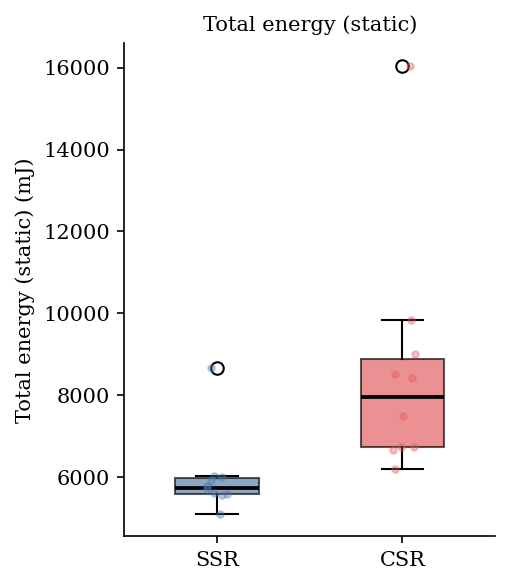
\includegraphics[width=0.32\linewidth]{../data/runs/20260401_143839/analysis/plots/static_energy_total_mj.png}\hfill
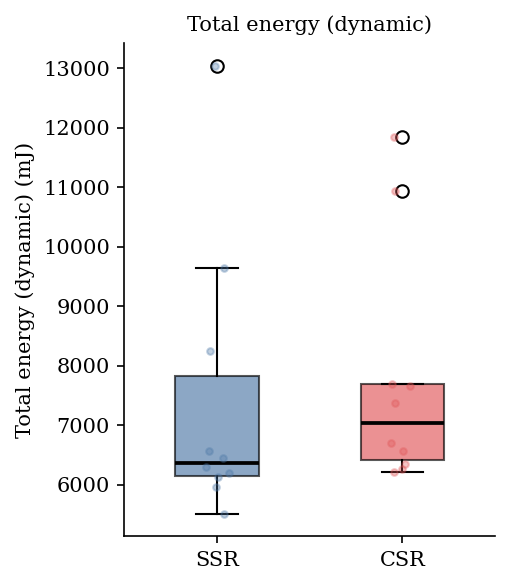
\includegraphics[width=0.32\linewidth]{../data/runs/20260401_143839/analysis/plots/dynamic_energy_total_mj.png}\hfill
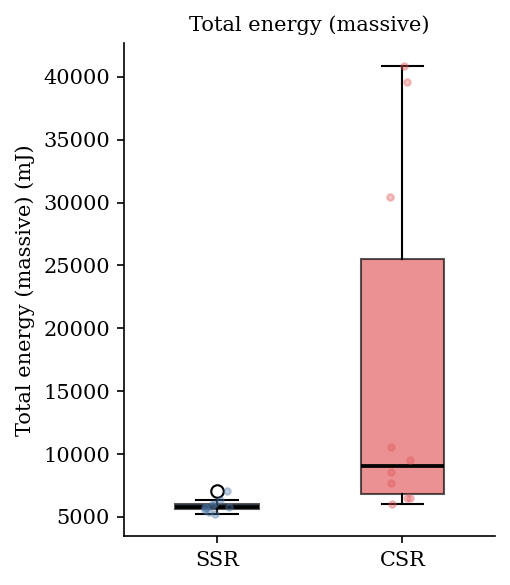
\includegraphics[width=0.32\linewidth]{../data/runs/20260401_143839/analysis/plots/massive_energy_total_mj.png}
\caption{Distribution plots for total energy in the corrected wireless benchmark, shown separately for the \textit{static}, \textit{dynamic}, and \textit{massive} scenarios. The \textit{massive} CSR condition shows the widest spread and the clearest high-energy outliers, while SSR remains comparatively compact in the \textit{static} and \textit{massive} scenarios.}
\label{fig:wireless-energy-distributions}
\end{figure}

Figure~\ref{fig:wireless-energy-distributions} shows the same pattern visually. The \textit{dynamic} scenario still shows substantial overlap between SSR and CSR despite the lower SSR median, whereas the \textit{static} and especially the \textit{massive} scenarios show a clearer separation in favour of SSR. The figure also shows that the main difference is not only the median level, but also the spread of the distributions. SSR remains relatively compact across scenarios, while CSR becomes much more variable as the workload increases, especially in the \textit{massive} scenario. In that condition, several CSR runs reach much higher energy values than the rest of the distribution, suggesting that client-side processing of the larger dataset was not only more energy-intensive in typical runs, but also less stable from run to run. This is one reason why a median-based interpretation is important in this dataset.

\begin{figure}[H]
\centering
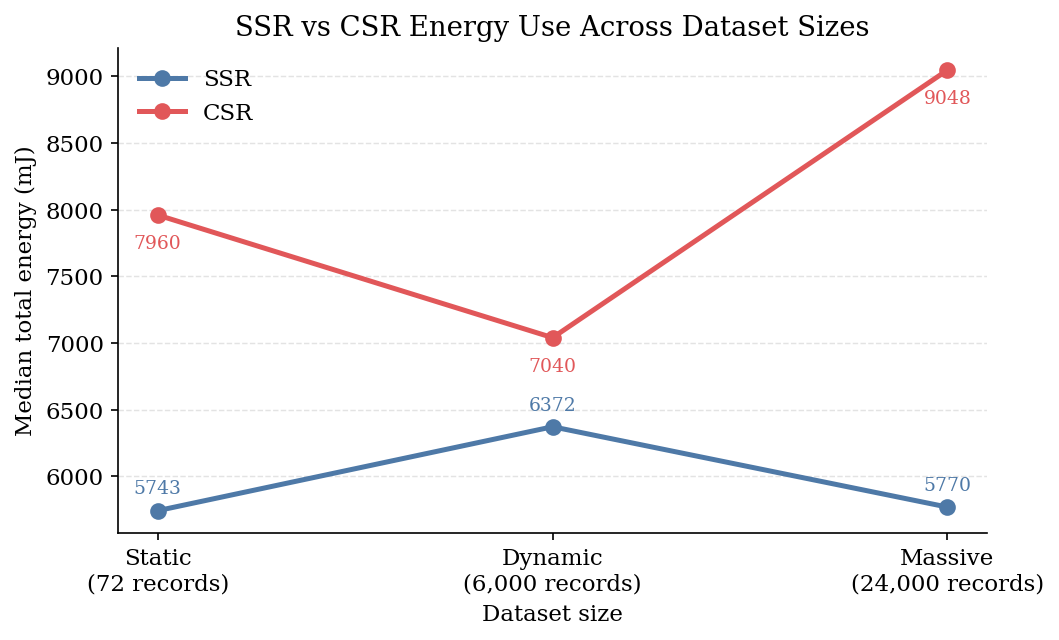
\includegraphics[width=0.82\linewidth]{../data/runs/20260401_143839/analysis/plots/energy_by_dataset_size_line.png}
\caption{Median total energy across the three dataset sizes used in the corrected wireless benchmark: \textit{static} (72 records), \textit{dynamic} (6{,}000 records), and \textit{massive} (24{,}000 records). The x-axis uses these scenario sizes on a log scale. SSR is shown in blue and CSR in red. The gap remains visible across all three scenarios and is widest in the \textit{massive} workload.}
\label{fig:energy-by-dataset-size-line}
\end{figure}

Figure~\ref{fig:energy-by-dataset-size-line} summarises the same energy comparison from a workload-growth perspective. It shows that SSR remains lower than CSR at 72, 6{,}000, and 24{,}000 records, with the largest separation appearing in the most data-heavy condition.

\begin{table}[htbp]
\centering
\caption{Selected browser and client-resource metrics for the corrected wireless benchmark. Medians are reported with IQR in parentheses.}
\label{tab:wireless-browser-summary}
{\small
\setlength{\tabcolsep}{4pt}
\begin{tabularx}{\linewidth}{@{}l l >{\RaggedRight\arraybackslash}X >{\RaggedRight\arraybackslash}X c@{}}
\toprule
\tablehead{Scenario} & \tablehead{Metric} & \tablehead{SSR median (IQR)} & \tablehead{CSR median (IQR)} & \tablehead{$p$} \\
\midrule
dynamic & LCP (ms) & 3302.0 (16.0) & 3270.0 (25.0) & 0.0010 \\
dynamic & FCP (ms) & 3302.0 (16.0) & 3270.0 (25.0) & 0.0010 \\
dynamic & TTFB (ms) & 31.2 (76.8) & 22.1 (46.0) & 0.1859 \\
dynamic & Navigation response size (KB) & 7.1 (0.0) & 3.9 (0.0) & $< 0.0001$ \\
dynamic & JS heap sample (MB) & 9.5 (0.0) & 9.5 (0.0) & 1.0000 \\
massive & LCP (ms) & 3296.0 (16.0) & 3274.0 (26.0) & 0.0532 \\
massive & FCP (ms) & 3296.0 (16.0) & 3274.0 (26.0) & 0.0532 \\
massive & TTFB (ms) & 67.8 (83.8) & 21.9 (139.4) & 0.1405 \\
massive & Navigation response size (KB) & 7.1 (0.0) & 3.9 (0.0) & $< 0.0001$ \\
massive & JS heap sample (MB) & 9.5 (0.0) & 13.6 (0.0) & $< 0.0001$ \\
static & LCP (ms) & 3292.0 (16.0) & 3290.0 (15.0) & 1.0000 \\
static & FCP (ms) & 3286.0 (18.0) & 3290.0 (15.0) & 0.6203 \\
static & TTFB (ms) & 24.1 (17.6) & 80.7 (135.0) & 0.9698 \\
static & Navigation response size (KB) & 7.2 (0.0) & 3.9 (0.0) & $< 0.0001$ \\
static & JS heap sample (MB) & 9.5 (0.0) & 9.5 (0.0) & 1.0000 \\
\bottomrule
\end{tabularx}
}
\end{table}

The browser-side metrics were more mixed than the energy results, as shown in Table~\ref{tab:wireless-browser-summary}. In the \textit{dynamic} scenario, CSR showed lower median LCP and FCP values than SSR (3270.0~ms versus 3302.0~ms for both metrics, $p = 0.0010$), and these differences met the corrected threshold. CSR also showed a lower median TTFB in the same scenario (22.1~ms versus 31.2~ms), but that difference did not meet the corrected threshold. In the \textit{massive} scenario, CSR again showed lower median LCP, FCP, and TTFB values, but none of those latency differences met the corrected threshold. In the \textit{static} scenario, the picture changed: LCP and FCP were effectively the same between conditions, and the CSR TTFB distribution was much more variable, producing a higher median than SSR.

One result was consistent across all three scenarios: the measured navigation response size was lower for CSR than for SSR, with medians of approximately 3.9~KB for CSR and 7.1--7.2~KB for SSR ($p < 0.0001$ in every scenario). This metric should be read as the size of the initial navigation response rather than the total transferred data for the full CSR route, because CSR also performs a follow-up inventory fetch after hydration. At the same time, Total Blocking Time and Cumulative Layout Shift remained at zero across all runs and therefore did not separate the two conditions. The JavaScript heap sample stayed equal at 9.5~MB in the \textit{dynamic} and \textit{static} scenarios. The clearest client-side resource difference appeared in the \textit{massive} scenario, where CSR reached a median heap sample of 13.6~MB compared with 9.5~MB for SSR ($p < 0.0001$). This matches the implementation difference in the prototype: CSR fetches raw inventory after hydration and performs the main data transformation step in the browser, whereas SSR performs that work before the page is delivered.

\begin{figure}[H]
\centering
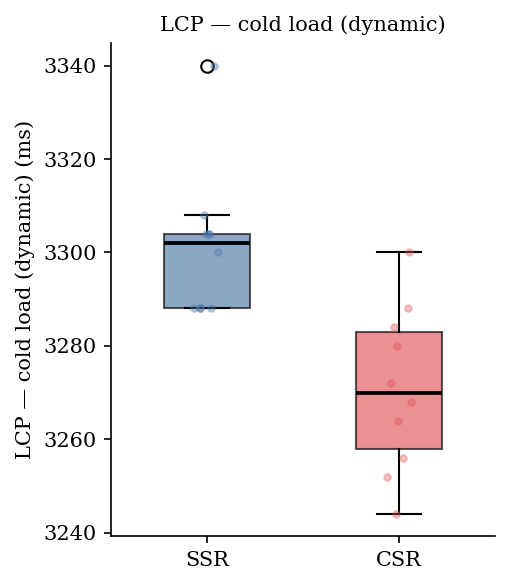
\includegraphics[width=0.32\linewidth]{../data/runs/20260401_143839/analysis/plots/dynamic_lcp_cold_ms.png}\hfill
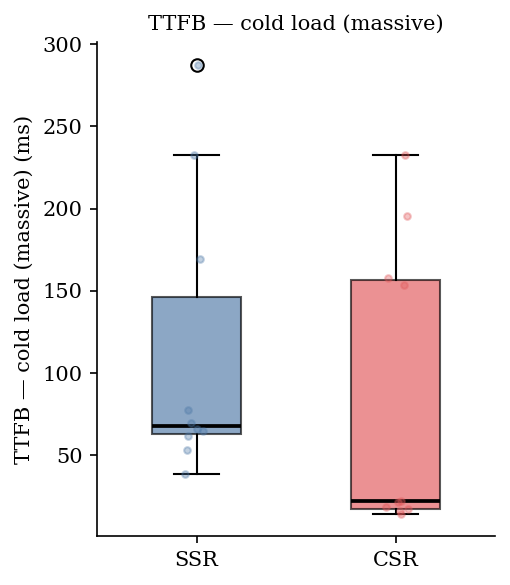
\includegraphics[width=0.32\linewidth]{../data/runs/20260401_143839/analysis/plots/massive_ttfb_cold_ms.png}\hfill
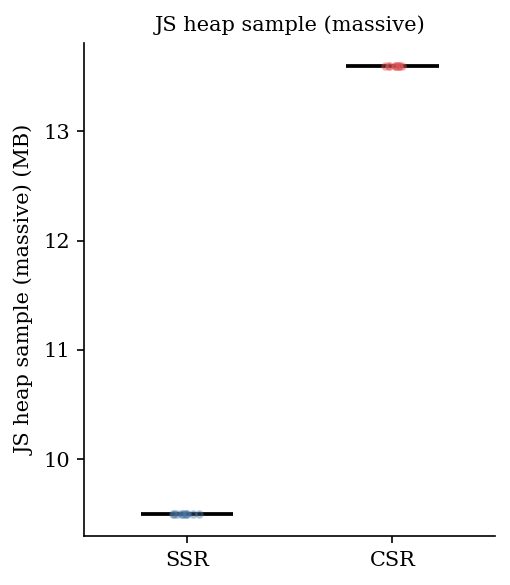
\includegraphics[width=0.32\linewidth]{../data/runs/20260401_143839/analysis/plots/massive_js_heap_mb.png}
\caption{Selected browser and client-resource distributions from the corrected wireless benchmark. From left to right: dynamic LCP, massive TTFB, and massive JavaScript heap sample. Together these plots illustrate the mixed pattern in the browser-facing metrics: CSR tends to show lower latency in some cases, while also incurring a larger browser-side memory footprint in the most data-heavy scenario.}
\label{fig:wireless-browser-distributions}
\end{figure}

Figure~\ref{fig:wireless-browser-distributions} illustrates this trade-off. The dynamic LCP plot shows a small but consistent latency advantage for CSR, the massive TTFB plot shows a directional tendency toward faster initial response in CSR without a decisive statistical result, and the massive heap plot shows that this pattern is accompanied by more browser-resident state when the client performs the larger processing workload itself.
